\section{Results}
	\subsection{Identification of enhancers and super-enhancers in vertebrate genomes}

		\begin{figure}[!h]
			\centering
			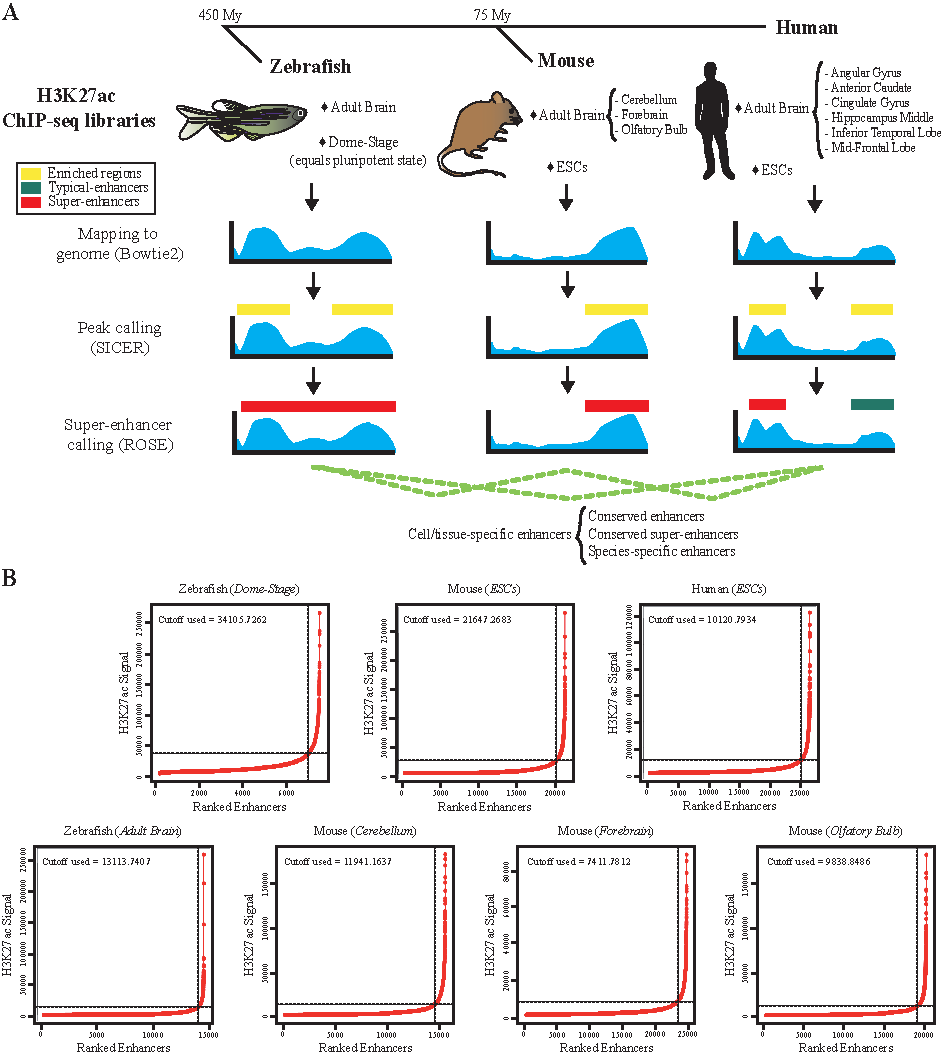
\includegraphics[width=16cm,height=18cm]{./figures/Figure_1.pdf}
  			\caption[Identification]{\textbf{Identification of enhancers in vertebrate genomes.} (A) H3K27ac ChIP-seq data sets analyzed and pipeline applied for the identification of typical-enhancers and super-enhancers. Evolutionary distances between the three organism are depicted in the upper dendrogram in million years (My). (B) Saturation curves of H3K27ac density across enhancers for the data sets analyzed in this study. The x-axis shows the number of ranked enhancers by density identified in each data set and their corresponding densities are plotted in the y-axis. Horizontal dot lines represent density cutoffs used for the identification of super-enhancers, and vertical dot lines demark super-enhancers from typical-enhancers.}
			\label{Identification}
			\rule{\textwidth}{0.25mm}
		\end{figure}

		The existence of long clusters of stretch enhancers in mammalian cells and tissues has previously been reported (Whyte et al., 2013; Lov\'en et al., 2013; Hnisz et al., 2013). These clusters of hyperactive chromatin or super-enhancers were originally identified based on ChIP-seq data that marked the genomic positions of master transcription factors in embryonic stem cells (ESCs) and Mediator sub-units (Whyte et al. 2013). However, it has been reported that the ChIP-seq data of additional transcriptional coactivators and histone marks might also contribute to the identification and refinement of super-enhancer locations. Specifically, the H3K27ac has been deamed as a robust epigenetic mark for predicting super-enhancers (Hnisz et al. 2013). Thus, to assess whether stretch enhancers are present outside of mammals and to create vertebrate maps of conventional enhancers further referred to as "typical-enhancers" and stretch enhancers further referred to as "super-enhancers", we based our predictions uniquely on zebrafish, mouse and human H3K27ac ChIP-seq data. For our analyses, we focused on the complex tissue of adult brain as well as ESC lines. We considered the early embryonic dome-stage of zebrafish as equivalent to the pluripotent state of mouse and human ESCs (Schier and Talbot, 2005; Vastenhouw et al., 2010).\\

		\begin{figure}[!h]
			\centering
			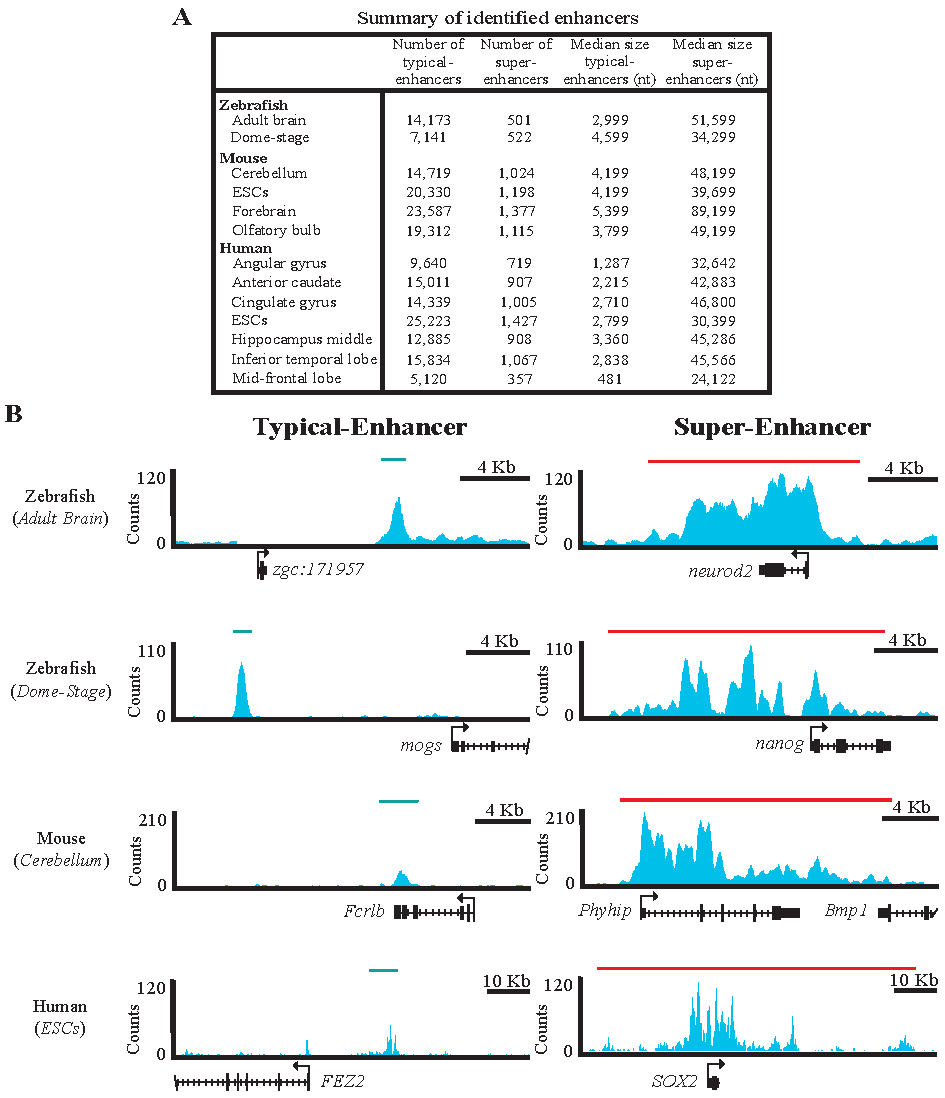
\includegraphics[width=16cm,height=18.6cm]{./figures/Figure_2.pdf}
  			\caption[Super-enhancers]{\textbf{Comparisons of typical-enhancers and super-enhancers.} (A) Summary table with the numbers of identified enhancers and their median sizes. (B) Genome tracks displaying examples of typical-enhancers and super-enhancers in the same data set for zebrafish, mouse and human. H3K27ac ChIP-seq profiles are shown in tag counts. Green and red bars over profiles represent typical-enhancers and super-enhancers respectively. Gene models are drawn below the binding profiles.}
			\label{Super-enhancers}
			\rule{\textwidth}{0.25mm}
		\end{figure}

		We took advantage of the available H3K27ac ChIP-seq data sets (Rada-Iglesias et al., 2011; Mouse ENCODE Consortium, 2012; Bogdanovic et al., 2012; Chadwick, 2012; Nord et al., 2013) and subjected them to a modified enhancer/super-enhancer computational identification pipeline following the same strategy used by Hnisz et al. (2013). Enhancer maps for the human adult brain data sets were already available (Hnisz et al., 2013), therefore, we used those published maps for all the analyses. Given that no zebrafish brain ChIP-seq data has been published, we generated H3K27ac ChIP profiles by sequencing two biological replicates prepared from whole adult brains of mixed genders. The included data sets and the pipeline applied for identification of typical-enhancers and super-enhancers are described in Figure 1A. First, we re-analyzed all available H3K27ac ChIP data sets by mapping the libraries to their corresponding reference genomes. Reads with low mapping quality were discarded from our further analyses. \texttt{SICER} was used to reveal genomic regions with H3K27ac enrichment (Zang et al., 2009), which represents regions of constitutive enhancers. Next, to classify constitutive enhancers as typical-enhancers or super-enhancers, we implemented the \texttt{ROSE} program (Whyte et al., 2013; Lov\'en et al., 2013). Briefly, \texttt{ROSE} stitches together neighboring constitutive enhancers using a maximal distance of 12.5 Kb creating long unique regions. After stitching, ChIP-seq densities are calculated for all regions and plotted by increasing density. To calculate the cutoff density to distinguish super-enhancers from typical-enhancers, the density value on the curve with a tangent equal to 1 is determined. This value represents the point at which the H3K27ac density starts to rapidly increase. All of the regions with a density higher than this value are considered as super-enhancers, while the remaining are classified as typical-enhancers (Figure 1B).\\

		Following this approach, We successfully identified super-enhancers in mouse, human and non-mammalian zebrafish data sets, and we found that zebrafish super-enhancers share key features with published mammalian super-enhancers such as their abundance and size (Figure 2A). For example, more enhancers were classified as typical-enhancer than as super-enhancer in all data sets and the median lengths of super-enhancers were longer than those of typical-enhancers. In general, super-enhancers spanned tens of thousands of base pairs, while typical-enhancers spanned only a few thousand base pairs (Figure 2B). It should be noted that with our approach we identified more super-enhancers for mouse ESCs than was originally reported (Whyte et al., 2013), 1198 versus 231, respectively. One possibility for this difference is that Whyte et al. first identified constitutive enhancers based on ChIP-seq data for Oct4, Sox2 and Nanog and then ranked them by Mediator signal, to refine their predictions. Nevertheless, based only on H3K27ac data we identified \(\sim79\)\% of the published super-enhancers, implying that by using uniquely this epigenetic mark and following our pipeline, it is possible to distinguish true super-enhancers from typical-enhancers.\\

	\subsection{Comparison of enhancer and super-enhancer attributes across vertebrates}

		To further assess if the main attributes characterizing mammalian typical-enhancers and super-enhancers were conserved across vertebrates, we first created metagene representations for all of the libraries analyzed (Figure 3A). These representations show the average H3K27ac density along typical-enhancers and super-enhancers in relation to their length. It is noticeable that for all data sets, the median size of typical-enhancers and super-enhancers differs by orders of magnitude and that super-enhancers accumulate most of the H3K27ac signal. Next, we investigated the correlation between H3K27ac density and length for the classification of super-enhancers. Although the correlation increased proportionally and the longest regions have higher densities, in some of the data sets there were long regions spanning up to 150 Kb with low H3K27ac density and subsequently were classified as typical-enhancers (Figure 3B).\\

		\begin{figure}[!h]
			\centering
			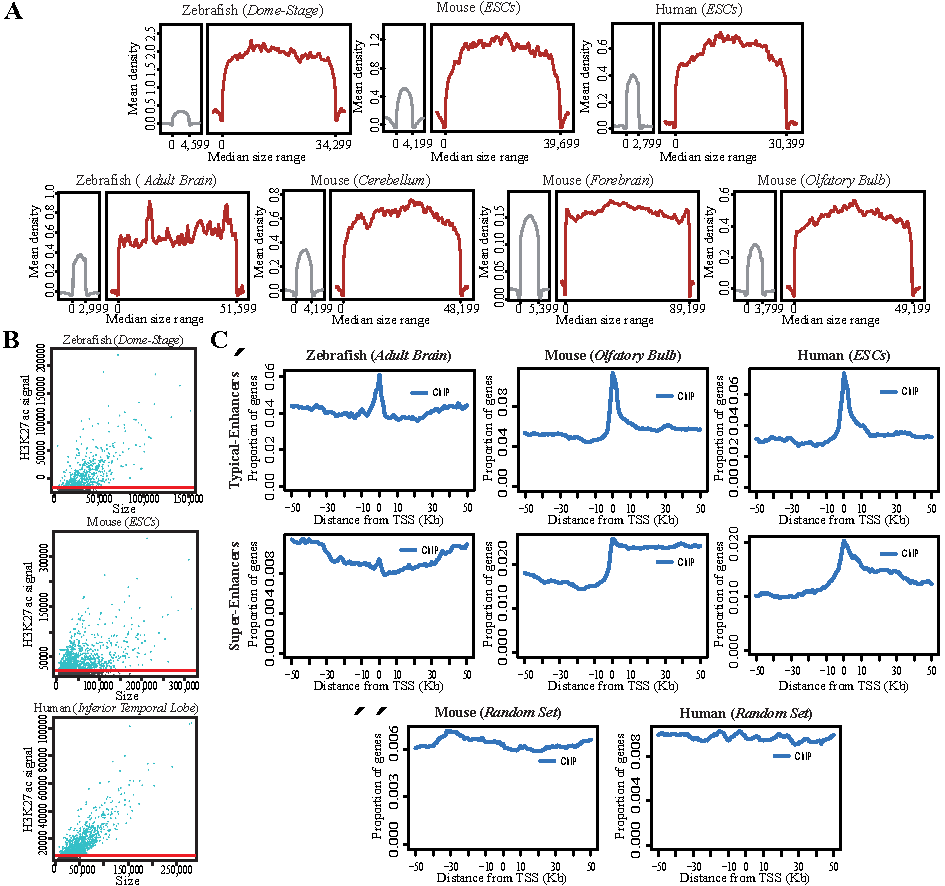
\includegraphics[width=16cm,height=15cm]{./figures/Figure_3.pdf}
  			\caption[Features]{\textbf{Representative features of vertebrate super-enhancers.} (A) Metagene representations of normalized H3K27ac density for typical-enhancers (grey curve) and super-enhancers (red curve). The y-axis shows the average H3K27ac density across enhancers. The regions displayed in the x-axis illustrate typical-enhancers and super-enhancers flanked by 3 Kb of adjacent sequence. Enhancer starts and ends are scaled relatively to median lengths. (B) Relationship between H3K27ac density (y-axis) and enhancer size (x-axis). Blue dots represent super-enhancers and the red line indicates the density cutoff used for the classification of enhancers. (C) Density plots with the proportion of genes for which the indicated locations around the TSS (x-axis) are covered by a typical-enhancer or a super-enhancer in the analyzed data sets (') and in randomly generated regions ('').}
			\label{Features}
			\rule{\textwidth}{0.25mm}
		\end{figure}

		It has also been noted that super-enhancers tend to overlap with the genes with which they are associated (Whyte et al., 2013; Lov\'en et al., 2013; Hnisz et al., 2013). Thus, we decided to examine if this tendency was maintained in our analyzed data sets. We observed that contrary to typical-enhancers, which cover the nearest regions surrounding the TSS, mouse and human super-enhancers tend to be more present in the down-stream region of the TSS. However, the distributions for zebrafish super-enhancers did not show the same tendency (Figure 3C). And given that only in 39 cases the distance between two super-enhancers was shorter than 100 Kb and the average distance was 2.2 Mb, the observed distribution could not be explained by problems with the stitching of adjacent super-enhancers around TSSs. Therefore, the distribution suggests that the relationship between super-enhancers and their target genes in zebrafish is different from that in mammals. Another explanation for this difference could be that it is a consequence of the incomplete gene annotation in zebrafish compared to that of mouse and human genomes. To eliminate the possibility that mouse and human super-enhancers were overlapping genes merely because of their long sizes, a random set of regions was analyzed for each genome. These random regions were not preferentially associated with a particular region within the 100 Kb window analyzed (Figure 3C).\\

	\subsection{Super-enhancers associate with cell-type specific genes}

		We annotated genes to typical-enhancers and super-enhancers following a strategy based on genomic proximity. Upon Gene Ontology (GO) enrichment analysis, we found that most of the annotated genes were related to development, neural processes and ESCs maintenance. As it has been reported by Whyte et al. (2013), Lov\'en et al. (2013) and Hnisz et al. (2013), the annotations for super-enhancers included key identity genes such as \textit{sox2}, \textit{nanog}, \textit{klf4}, \textit{wnt11}, \textit{prdm14}, \textit{foxh1}, and \textit{ptch2} (Heisenberg et al., 2000; Takahashi and Yamanaka, 2006; Burton et al., 2013; Holtz et al., 2013; Takahashi et al., 2014) in the ESCs data sets. By contrast, in the brain data sets we found identity genes involved in neural development, synaptic communication and neural stem quiescence such as \textit{neurod2}, \textit{neurexin1}, \textit{nfix}, \textit{zic1} and \textit{zic4} (Rissone et al., 2007; Eisen et al., 2008; Sato and Takeda, 2013; Martynoga et al., 2013). Interestingly, the three genes coding for the master transcription factors in ESCs were only associated with super-enhancers in the mouse ESCs data set, while in the zebrafish data set only \textit{nanog} was associated with a super-enhancer and the other two genes were associated with typical-enhancers. We found that in the human ESCs, only \textit{SOX2} and \textit{NANOG} had super-enhancers associated with them and, strikingly, the 6 Mb region surrounding \textit{OCT4} was depleted of H3K27ac signal, a result that we reproduced using another two independent human ESCs data sets (Chadwick, 2012; Loh et al., 2014; data not shown).\\

		To investigate whether the key identity genes that we identified were uniquely associated to a super-enhancer in adult brain or ESCs but not in the other cell/tissue type, we focused on three examples of key identity genes with a conserved super-enhancer in zebrafish, mouse and human. We selected the forkhead transcription factor \textit{foxh1} for ESCs and the couple \textit{zic1} and \textit{zic4} for adult brain data sets. It has been reported that FOXH1 is able to enhance the efficiency of reprogramming of human differentiated cells to generate induced pluripotent stem cells (Takahashi et al., 2014). Although no super-enhancers were associated to this gene in the brain, we found that in ESCs of all three organisms, the super-enhancer was present and overlapped the entire gene body of \textit{foxh1}. Only in mouse cerebellum, two typical-enhancers were found in the neighboring area (Figure 4A). On the other hand, expression of \textit{zic1} and \textit{zic4} is required for the normal morphogenesis of the hindbrain ventricle controlled by proliferation and fate specification in zebrafish (Eisen et al., 2008). Our data showed that, similar to \textit{foxh1}, brain super-enhancers covered the entire gene body of both \textit{zic1} and \textit{zic4}  and spanned through the up-stream and down-stream regions. By contrast, in zebrafish, mouse and human ESCs these genes were associated with typical-enhancers, suggesting that \textit{zic1} and \textit{zic4} might also be expressed in ESCs but its expression might not be as essential as in the brain (Figure 4B).\\

		\begin{figure}[!h]
			\centering
			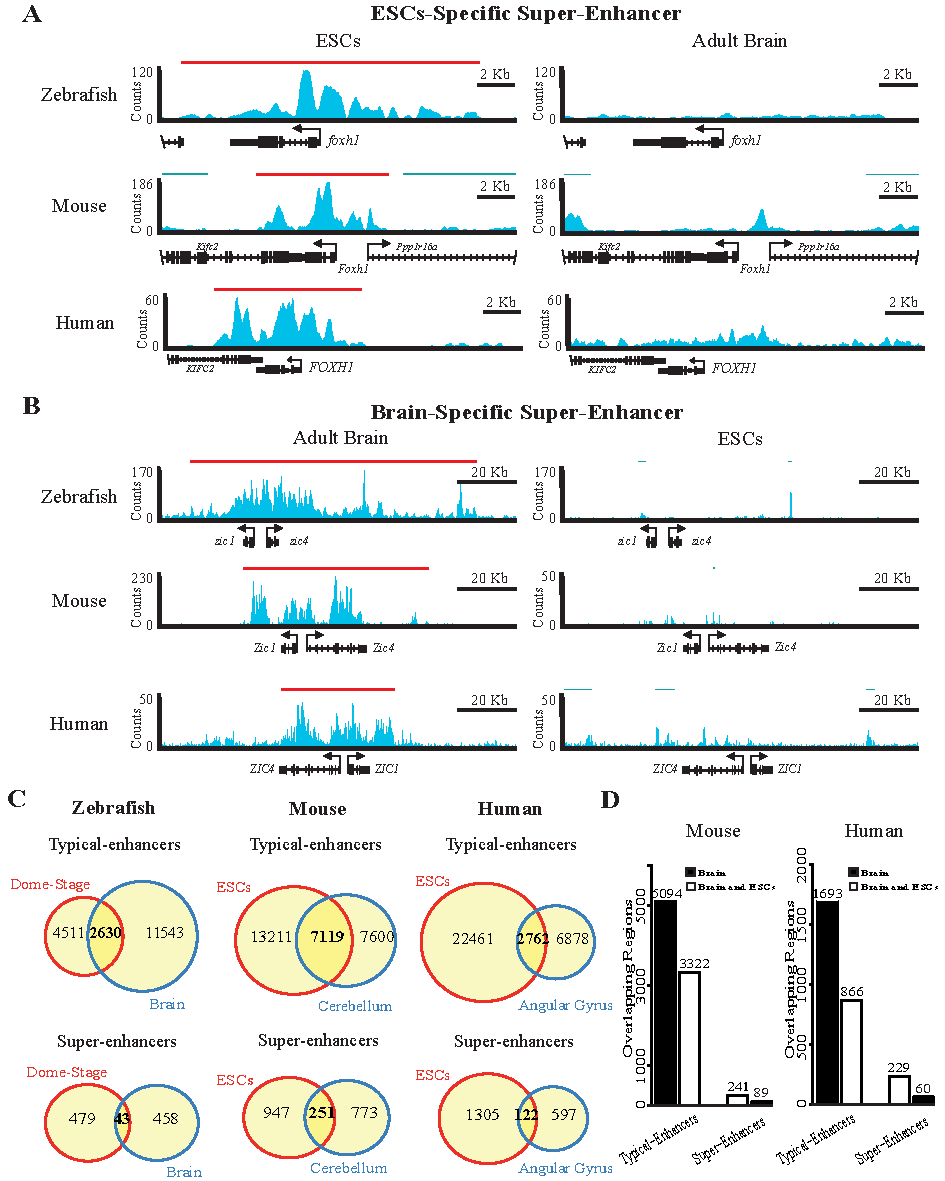
\includegraphics[width=15cm,height=17cm]{./figures/Figure_4.pdf}
  			\caption[Specificity]{\textbf{Significant fractions of enhancers and super-enhancers are cell/tissue-specific.} (A) Examples of identity genes associated with a super-enhancer across vertebrates. Genome tracks are displayed as described in Figure 2B. (B) Venn diagrams with the global overlaps of typical-enhancers and super-enhancers in the different data sets. (C) Barplots representing the number of enhancer overlapping regions among brain data sets (black bar) or among brain and ESCs data sets (white bar) for mouse and human.}
			\label{Specificity}
			\rule{\textwidth}{0.25mm}
		\end{figure}

		Next, we globally compared typical-enhancers and super-enhancers between adult brain and ESCs. To obtain the sets of overlapping regions in the genomes, we compared the maps of typical-enhancers and super-enhancers between data sets from the same organism. We observed that for zebrafish, mouse and human, the number of overlapping regions is higher for typical-enhancers than for super-enhancers (Figure 4C). This observation is consistent with the idea that super-enhancers are generally associated with cell-type specific genes and thus, we would expect that only a small subset of super-enhancers are shared between different cell types. Specifically, we expected that some genes coding for transcriptional cofactors such as Mediator would be associated with super-enhancers in different cell-types. Given that for mouse and human, data sets for different brain regions are available, we performed multiple comparisons of the typical-enhancer and super-enhancer maps to obtain a global panorama of brain enhancers compared with ESCs enhancers. As seen in the pairwise comparisons, the number of overlapping regions among the typical-enhancers was higher than for super-enhancers in mouse and human. It also should be noted that, in general, the number of overlapping regions between different brain data sets is higher than for overlapping regions between brain and ESC data sets (Figure 4D). This data supports the idea that the enhancer landscape changes according to cell types and that the subset of enhancers and super-enhancers identified and analyzed is highly specific to that particular cell type or tissue.\\

	\subsection{Conservation of enhancers and super-enhancers in vertebrate genomes}

		\begin{figure}[!h]
			\centering
			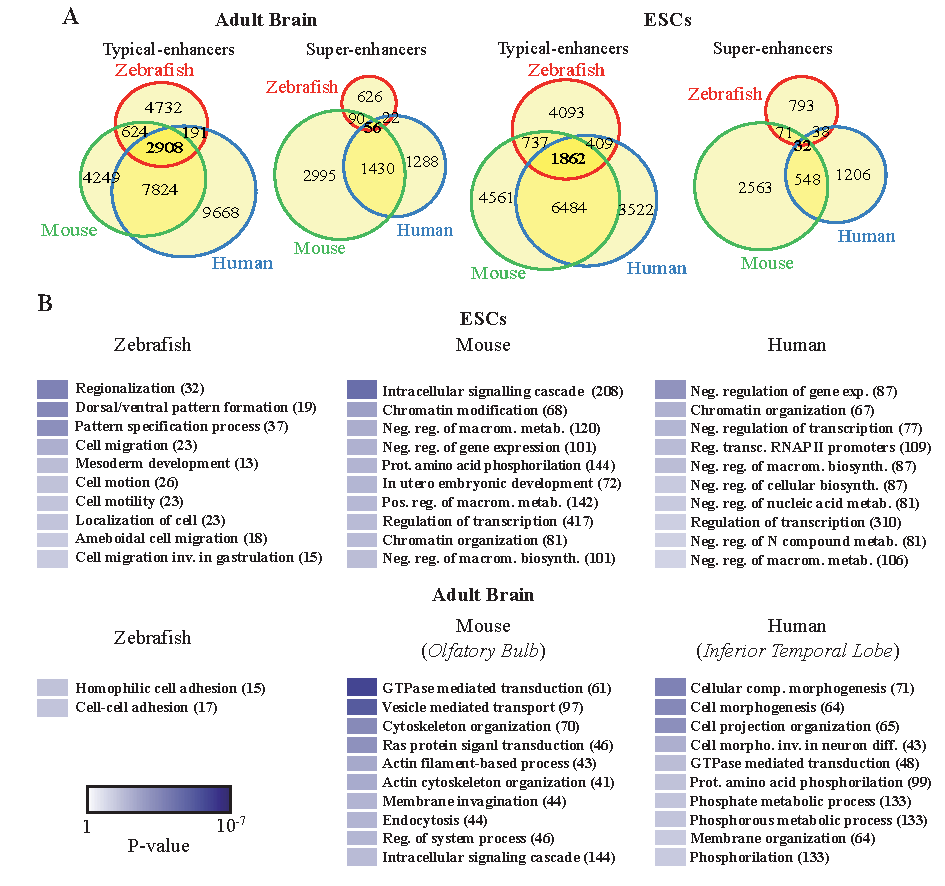
\includegraphics[width=16cm,height=16cm]{./figures/Figure_5.pdf}
  			\caption[Conservation]{\textbf{Conservation of enhancer and super-enhancer target genes and functions across vertebrate genomes.} (A) Venn diagrams displaying the overlaps of enhancer maps for zebrafish, mouse and human. (B) Top ten molecular function GO terms enriched for genes associated with super-enhancers. Adjusted p-values for the GO terms are displayed in a color scale. Only terms with adjusted p-values $<0.06$ are considered as significantly enriched.}
			\label{Conservation}
			\rule{\textwidth}{0.25mm}
		\end{figure}

		Taking into account that super-enhancers are associated with genes that specify cell identity and also the fact that most of these key regulator genes are conserved across organisms, we next investigated if typical-enhancers and super-enhancers were associated with the same genes across vertebrates. We performed inter-species comparisons based on gene name and found that, among enhancer maps, both typical-enhancers and super-enhancers for the same genes were conserved. For the adult brain and ESCs comparisons, more genes associated with typical-enhancers (2908 for adult brain and 1862 for ESCs) than with super-enhancers (56 for adult brain and 32 for ESCs) were shared between zebrafish, mouse and human. The conservation of enhancer-associated target genes was higher between mouse and human than when they were compared to zebrafish (Figure 5A), consistent with the evolutionary distance among these species. The lists of common genes associated with a super-enhancer included those related to cell fate identity such as \textit{nfix}, \textit{foxh1}, \textit{neurod2} and \textit{sox2}. In addition, genes that code for transcriptional coactivators were also present among these lists, which is logical considering that super-enhancers are highly occupied by transcriptional cofactors. High levels of these proteins are required in the cell, and it has been reported that super-enhancers can trigger higher rates of transcription than typical-enhancers (Whyte et al., 2013), which could explain the association of super-enhancers to those genes. It should be noted that the comparisons were performed only based on the gene name. Thus, the observed overlaps are likely an underestimation of the real conservation because ortholog genes do not always share the same gene name.\\

		An alternative strategy to determine the conservation of super-enhancers is to analyze if the biological processes with which their associated genes are involved, remain similar in zebrafish, mouse and human. We performed GO enrichment analysis and found that ESCs data sets were mainly enriched for terms relative to transcription regulation, while for the dome-stage data set the top terms were related to patterning and cell migration. For the adult brain data sets, among the top terms cytoskeleton organization, morphogenesis and cell-adhesion (Figure 5B). Although the terms found for the zebrafish brain data set were similar to those found for the mouse and human data sets, only two of the terms had significant adjusted p-values. Most likely, this is a consequence of the zebrafish background that is considered by the program used for the enrichment of GO terms, as only a reduced number of terms got significant p-values also for the dome-stage data set. For all data sets in zebrafish, mouse and human, we found that transcription regulator activity was among the top molecular function terms. These results highlight the frequent associations that exist between super-enhancers and regulators of transcription.\\

